\def\QRCODE{TB_IPR_TUT.IMG.boolean_models_matlab_tempqrcode.png}
\def\QRPAGE{http://www.iptutorials.science/tree/master/TB_IPR/TUT.IMG.boolean_models/matlab/temp}
\mcorrectionsection{Matlab correction}

%\begin{mcomment}
\begin{mremark}
%Please notice that when using boolean arrays in matlab, the notations $1-X$ and $\sim X$ are equivalent. When using uint8 arrays, verify that the values range into [0;1].
%\end{mremark}
\end{mcomment}

\subsection{Simulation of a 2-D Boolean model}

Here is the function for generating an isotropic Boolean model of rectangular grains:
\begin{matlab}
function [BM] = BMgenerationRectangle(Wsize,Gamma,WidthLaw,LengthLaw)
% Simulation of an isotropic boolean model with rectangular grains

% INPUT:
    % Wsize: dimensions of the observation window in which the model is generated
    % Gamma: intensity of the germ process
    % WidthLaw: parameters of the Gaussian law governing the width of the grains.
    % LengthLaw: parameters of the Gaussian law governing the length of the grains.

% OUTPUT: a structure BM
    % BM.Polygons: set of polygons as a realization of the boolean model observed in a window of size Wsize
    % BM.GrainNumber: number of grains
    % BM.GrainLocation: location of germs
    % BM.GrainSize: size of grains
    % BM.GrainOrientation: orientations of grains


% EXAMPLE:
    % Wsize = [512 512];
    % Gamma = 100/Wsize(1)/Wsize(2);
    % WidthLaw = [30 10]; 
    % LengthLaw = [50 20];
    % [BM] = BMgenerationRectangle(Wsize,Lambda,WidthLaw,LengthLaw);

%%%%%%%%%%%%%%%%%%%%%%%%%%%%%%

% generate the observation window as polygon
Wx = [0 Wsize(1) Wsize(1) 0 0];
Wy = [0 0 Wsize(1) Wsize(1) 0];

% generate edge correction
widthEdgeEffect = WidthLaw(1)+2*WidthLaw(2);
lengthEdgeEffect = LengthLaw(1)+2*LengthLaw(2);
edgeEffect = round(sqrt(widthEdgeEffect^2 + lengthEdgeEffect^2));

% generate the germs of the grains
grainLocation = BMgrainLocation(Wsize, edgeEffect, Gamma);
nbGrain = size(grainLocation,1);

% generate the width/length of the grains
grainWidth = BMgrainSize(nbGrain,WidthLaw);
grainLength = BMgrainSize(nbGrain,LengthLaw);

% generate the orientation of the grains
grainOrientation =  unifrnd(0,180,1,nbGrain);

% generate the frame with the grains
l = [];
L = [];
x = [];
y = [];
ang = [];
nb = 0;

X=[];
Y=[];

for i = 1:nbGrain 

    [X0,Y0] = generationRectanglePolygon(grainLocation(i,1),grainLocation(i,2),grainWidth(i),grainLength(i),grainOrientation(i));
          
    % does the grain intersect Wo?
    [Xtemp,Ytemp] = polybool('intersection',X0,Y0,Wx,Wy);
    
    if ~isempty(Xtemp)
        [X,Y] = polybool('union',X,Y,Xtemp,Ytemp);
        l = [l grainLength(i)];
        L = [L grainWidth(i)];
        x = [x grainLocation(i,1)];
        y = [y grainLocation(i,2)];
        ang = [ang grainOrientation(i)];
        nb = nb+1;
        
    end

end
    
BM = struct('GrainSize',{[l;L]},'GrainLocation',{[x;y]},'Polygons',{[X;Y]},...
'GrainOrientation',{ang},'GrainNumber',{nb});

end
\end{matlab}
\begin{matlab}
function [locationGrain] = BMgrainLocation(Wsize, edgeEffect, gamma)

nf = Wsize(1) + edgeEffect;
nc = Wsize(2) + edgeEffect;
areaW = nf*nc;
n = poissrnd(gamma*areaW);

xn = rand(1,n)*nf - edgeEffect/2;
yn = rand(1,n)*nc - edgeEffect/2;
locationGrain = [xn',yn'];

end
\end{matlab}
\begin{matlab}
function  [sizeGrain] = BMgrainSize(nbGrain, paramGrain_size)

sizeGrain = normrnd(paramGrain_size(1),paramGrain_size(2),1,nbGrain); %mu, std
%ignoring values less or equal to 0
indices = find(sizeGrain<=0);
while isempty(indices)==0
    temp = normrnd(paramGrain_size(1),paramGrain_size(2),length(indices),1);
    sizeGrain(indices) = temp;
    indices = find(sizeGrain<=0);
end;

end
\end{matlab}
\begin{matlab}
function [x,y] = generationRectanglePolygon(x0,y0,a,b,theta)

% INPUT
% (x0,y0): center coordinates of the rectangle
% (a,b): width and length of the rectnagle
% theta: orientation of the rectange
%
% OUTPUT
% (x,y): coordinates of the polygon / corners of the polygon

thetaRadians = theta*pi/180;
R = [cos(thetaRadians) -sin(thetaRadians);sin(thetaRadians) cos(thetaRadians)];
t = [x0;y0];
z1 = R*[a/2;-b/2] + t;
z2 = R*[a/2;b/2] + t;
z3 = R*[-a/2;+b/2] + t;
z4 = R*[-a/2;-b/2] + t;

z = [z1,z2,z3,z4,z1];
x = z(1,:);
y = z(2,:);

end
\end{matlab}
\noindent Notice the use of the Matlab function \minline{polybool} to make the union of polygons.\\
\noindent Then, you can execute the following code to simulate and visualize a realization of such a process:
\begin{matlab}
% parameters
Wsize = [500 500];
Gamma = 100/Wsize(1)/Wsize(2);
WidthLaw = [30 10]; 
LengthLaw = [50 20];

% generation
warning off;
[BM] = BMgenerationRectangle(Wsize,Gamma,WidthLaw,LengthLaw);

% visualization
BMshow(BM.Polygons);
axis off
axis([0 500 0 500]);
\end{matlab}
\noindent The function \minline{BMshow} has been given for this tutorial:
\begin{matlab}
function BMshow(xy)

x=xy(1,:);
y=xy(2,:);
[xcells,ycells] = polysplit(x,y);
n = length(xcells);

cc = zeros(n,1);
for i=1:n
   cc(i) = ispolycw(xcells{i},ycells{i});
end

color=[0.5 0.5 0.5];
for i=1:n
   if cc(i)==1
       p = patch(xcells{i},ycells{i},color);
       set(p,'EdgeColor','k','LineWidth',1);
   else
       p = patch(xcells{i},ycells{i},'w');
       set(p,'EdgeColor','k','LineWidth',1);
   end
end

axis square;axis equal;
\end{matlab}
\noindent with the following resulting image:
\begin{figure}[htbp]
 \centering
 %\subfloat[Original image.]{
 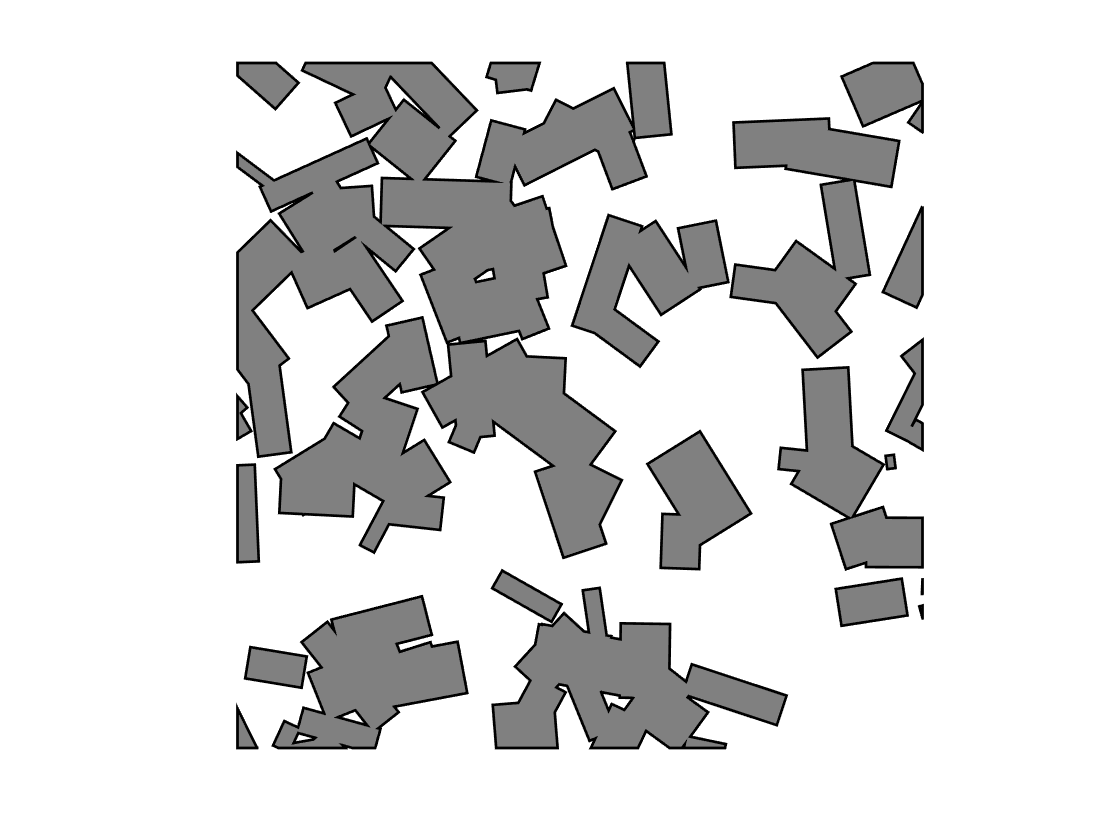
\includegraphics[width=10cm]{BMrectangles.png}\label{fig:boolean_models:matlab:BMrectangles}
 %}\hspace*{1cm}
 
 \caption{Realization of an isotropic Boolean model of rectangular grains.}
\end{figure}

\subsection{Geometrical characterization of a 2-D Boolean model}
You can use the given function \minline{BMminkowskyDensities} 
\begin{matlab}
function [area, per, chi] = BMminkowskiDensities(xy, Wsize)
% INPUT:
  % BM: boolean model in a bounded observation window

% OUTPUT:
  % per: density of perimeter 
  % area: density of area 
  % chi: density of euler characteristic
  
Warea = Wsize(1)*Wsize(2);
Wperimeter = 2*(Wsize(1)+Wsize(2));

x=xy(1,:);
y=xy(2,:);
[xcells,ycells] = polysplit(x,y);
n = length(xcells);

cc = zeros(n,1);
for i=1:n
   cc(i) = ispolycw(xcells{i},ycells{i});
end
  
% Compute Minkowski densities (Weil's formulae)
area = PolyArea(xcells,ycells,cc)/Warea;

per = (PolyPerimeter(xcells,ycells)/Warea) - (Wperimeter*area/Warea);

chi = (PolyEuler(cc)/Warea) - (1/2/pi)*(Wperimeter*PolyPerimeter(xcells,ycells)/Warea/Warea) + ...
  ((1/2/pi)*((Wperimeter^2)/(Warea^3) )- 1/Warea/Warea)*area*Warea;

end
\end{matlab}
\begin{matlab}
function [area] = PolyArea(xcells,ycells,cc)

n = length(xcells);
area=0;

%axis square;axis equal;
for i=1:n
   if cc(i)==1 % true polygon
       area = area + polyarea(xcells{i},ycells{i});
   else % hole
       area = area - polyarea(xcells{i},ycells{i});
   end
end 

end
\end{matlab}
\begin{matlab}
function [per] = PolyPerimeter(xcells,ycells)
% compute perimeter of polygons
n = length(xcells);

for i=1:n
    x=xcells{i};
    y=ycells{i};
    j=1;
    z(i)=0;
    while j<length(x)
        z(i)=z(i)+ norm([(x(j+1)-x(j)),(y(j+1)-y(j))],2);
        j=j+1;
    end
end

per = sum(z);

end
\end{matlab}
\begin{matlab}
function [chi] = PolyEuler(cc)
% compute Euler characteristic of polygons
chi = 2*sum(cc)-length(cc);

end
\end{matlab}
\noindent to compute the densities of the area, perimeter and Euler characteritics on different realizations of this 2-D Boolean model:
\begin{matlab}
% computation of the Minkowski densities on different realizations
nbRealizations = 20;
W = zeros(nbRealizations,3);

for i=1:nbRealizations
    [BM] = BMgenerationRectangle(Wsize,Gamma,WidthLaw,LengthLaw);
    [area, per, chi] = BMminkowskiDensities(BM.Polygons,Wsize);
    W(i,:) = [area, per/2, chi*pi];
    clear area per chi;
end
\end{matlab}
\noindent and by inverting the Miles formulas:
\begin{matlab}
% mean densisties
W = mean(W,1);

% inversion of the Miles formulas
Gamma_num = 1/pi * (W(3)/(1-W(1)) + W(2)^2/((1-W(1))^2) );
Area_num = 1/Gamma_num * (-log(1-W(1)));
Per_num = 1/Gamma_num * ( W(2)/(1-W(1)) );
\end{matlab}
\noindent Now, you can compare these estimated values with the theoretical ones (the parameters of the model are known!):
\begin{matlab}
% theoretical values
Area = WidthLaw(1)*LengthLaw(1);
Per = (WidthLaw(1)+LengthLaw(1));

% comparison
error_Gamma = abs(Gamma_num-Gamma)/Gamma;
error_Area = abs(Area_num-Area)/Area;
error_Per = abs(Per-Per_num)/Per;
\end{matlab}
Here are the results for 20 specific realizations:
\begin{sh}
errorGamma = 0.0141
errorArea = 0.0071
errorPer = 0.0049
\end{sh}

